%%%%%%%%%%%%%%%%%%%% book.tex %%%%%%%%%%%%%%%%%%%%%%%%%%%%%
%
% sample root file for the chapters of your "monograph"
%
% Use this file as a template for your own input.
%
%%%%%%%%%%%%%%%% Springer-Verlag %%%%%%%%%%%%%%%%%%%%%%%%%%


% RECOMMENDED %%%%%%%%%%%%%%%%%%%%%%%%%%%%%%%%%%%%%%%%%%%%%%%%%%%
\documentclass[graybox,envcountchap,sectrefs]{svmono}

% choose options for [] as required from the list
% in the Reference Guide

\usepackage{amsfonts}
\usepackage{mathptmx}
\usepackage{helvet}
\usepackage{courier}
%
\usepackage{type1cm}         

\usepackage{makeidx}         % allows index generation
\usepackage{graphicx}        % standard LaTeX graphics tool
                             % when including figure files
\graphicspath{{Figures/}}
\usepackage{multicol}        % used for the two-column index
\usepackage[bottom]{footmisc}% places footnotes at page bottom

% see the list of further useful packages
% in the Reference Guide

\makeindex             % used for the subject index
                       % please use the style svind.ist with
                       % your makeindex program
    \addtolength{\oddsidemargin}{-1.25in}
 	\addtolength{\evensidemargin}{-1in}
	\addtolength{\textwidth}{2.5in}

	\addtolength{\topmargin}{0in}
	\addtolength{\textheight}{1.5in}
%%%%%%%%%%%%%%%%%%%%%%%%%%%%%%%%%%%%%%%%%%%%%%%%%%%%%%%%%%%%%%%%%%%%%

\begin{document}

\author{R. C. Gunning}
\title{Lectures on Riemann Surfaces}
\subtitle{I}
\maketitle

\frontmatter%%%%%%%%%%%%%%%%%%%%%%%%%%%%%%%%%%%%%%%%%%%%%%%%%%%%%%
\newcommand{\N}{\mathbb{N}}

\newcommand{\Q}{\mathbb{Q}}
\newcommand{\Z}{\mathbb{Z}}

\newcommand{\C}{\mathbf{C}}
\newcommand{\PP}{\mathbf{P}}
\newcommand{\HHH}{\mathbf{H}}
\newcommand{\DD}{\mathbf{D}}
\newcommand{\R}{\mathbf{R}}

\newcommand{\OO}{\mathcal{O}}
\newcommand{\B}{\mathcal{B}}
\newcommand{\cU}{\mathcal{U}}
\newcommand{\F}{\mathcal{F}}



\newcommand{\rO}{\mathrm{O}}
\newcommand{\op}{\mathrm{op}}
\newcommand{\rd}{~\mathrm{d}} %roman d
\newcommand{\GL}{\mathrm{GL}}
\newcommand{\SU}{\mathrm{SU}}
\newcommand{\SL}{\mathrm{SL}}
\newcommand{\SO}{\mathrm{SO}}
\newcommand{\U}{\mathrm{U}}
\newcommand{\Sp}{\mathrm{Sp}}
\newcommand{\im}{\mathrm{Im}}
\newcommand{\ord}{\mathrm{ord}}
\newcommand{\End}{\mathrm{End}}
\newcommand{\Aut}{\mathrm{Aut}}
\newcommand{\Hom}{\mathrm{Hom}}
\newcommand{\ad}{\mathrm{ad}}
\newcommand{\tr}{\mathrm{tr}}
\newcommand{\Rad}{\mathrm{Rad}}



% \newcommand{\DD}{\overline{\mathbf{D}}}


\newcommand{\res}{\mathsf{res}}



% %%%%%%%%%%%%%%%%%%%%%%% dedic.tex %%%%%%%%%%%%%%%%%%%%%%%%%%%%%%%%%
%
% sample dedication
%
% Use this file as a template for your own input.
%
%%%%%%%%%%%%%%%%%%%%%%%% Springer %%%%%%%%%%%%%%%%%%%%%%%%%%

\begin{dedication}
Use the template \emph{dedic.tex} together with the Springer document class SVMono for monograph-type books or SVMult for contributed volumes to style a quotation or a dedication\index{dedication} at the very beginning of your book in the Springer layout
\end{dedication}





% %%%%%%%%%%%%%%%%%%%%%%foreword.tex%%%%%%%%%%%%%%%%%%%%%%%%%%%%%%%%%
% sample foreword
%
% Use this file as a template for your own input.
%
%%%%%%%%%%%%%%%%%%%%%%%% Springer %%%%%%%%%%%%%%%%%%%%%%%%%%

\foreword

%% Please have the foreword written here
Use the template \textit{foreword.tex} together with the Springer document class SVMono (monograph-type books) or SVMult (edited books) to style your foreword\index{foreword} in the Springer layout. 

The foreword covers introductory remarks preceding the text of a book that are written by a \textit{person other than the author or editor} of the book. If applicable, the foreword precedes the preface which is written by the author or editor of the book.


\vspace{\baselineskip}
\begin{flushright}\noindent
Place, month year\hfill {\it Firstname  Surname}\\
\end{flushright}



%%%%%%%%%%%%%%%%%%%%%%preface.tex%%%%%%%%%%%%%%%%%%%%%%%%%%%%%%%%%%%%%%%%%
% sample preface
%
% Use this file as a template for your own input.
%
%%%%%%%%%%%%%%%%%%%%%%%% Springer %%%%%%%%%%%%%%%%%%%%%%%%%%

\preface

%% Please write your preface here
These are notes for a course of lectures given at Princeton University during the academic year 1965-66. The subject of the lecture was compact Riemann surfaces, considered as complex analytic manifolds. There are already several expositions of this subject from basically the same point of view; the foremost is undoubtedly Hermann Weyl's ``Die Idee der Riemannschen Fl\"ache, (The Idea of the Riemann Surface)'' and most of the later treatments have followed Weyl's approach to a large degree. During recent years there has been considerable activity in the study of complex analytic manifolds of several dimensions, and various new tools and approaches have been developed. The aim of the lectures, in addition to treating of a beautiful subject for its own sake, was to introduce the students to some of these techniques in the case of one complex variable, where things are simpler and the results more complete.\par

The material covered is indicated by the table of contents. No familiarity with manifolds, sheaves, or sheaf cohomology was assumed, so those subjects are developed ab initio (from the beginning), although only so far as necessary for the purposes of the lectures. On the other hand, no attempt was made to discuss in detail the topology of surfaces; for that is really another subject, and there are very good treatments available elsewhere. The basic analytic tool used was the Serre duality theorem, rather than the theory of harmonic integrals or harmonic functions. The detailed treatment of the analytic properties of compact Riemann surfaces begins only in Chapter VII. Unfortunately, there was not enough time to get very far in the discussions; os the lectures have the air of being but an introduction to the subject. This may explain some of the surprising omissions, also. I hope to have an opportunity to continue the discussion further sometime.\par

With the possible exception of parts of Chapter IX, there is nothing really new here. References to the literature are scattered throughout, with no attempt at completeness. In addition to these and to the book of Hermann Weyl, the following general references should be mentioned here: Paul Appell and Edouard Goursat, ``Th\'eorie des Functions Alg\'ebriques,'' (gauthier-Villars, 1930); Kurt Hensel and Georg Landsberg, ``Theorie der algebraischen Funktionen einer Variablen,'' (Teubner, 1902; Chelsea, 1962); and Jean-Pierre, ``Corps locaux,'' (Hermann, 1962).\par

I should like to express my thanks here to Richard Hamilton, Henry Laufer, and Richard Mandelbaum for many suggestions and improvements; and to Elizabeth Epstein for typing the manuscript.

 

 \vspace{\baselineskip}
 \begin{flushright}\noindent
 Princeton, New Jersey,\hfill {\it R. C. Gunning}\\
 May, 1966 \hfill \\
 \end{flushright}



% %%%%%%%%%%%%%%%%%%%%%%acknow.tex%%%%%%%%%%%%%%%%%%%%%%%%%%%%%%%%%%%%%%%%%
% sample acknowledgement chapter
%
% Use this file as a template for your own input.
%
%%%%%%%%%%%%%%%%%%%%%%%% Springer %%%%%%%%%%%%%%%%%%%%%%%%%%

\extrachap{Acknowledgements}

Use the template \emph{acknow.tex} together with the Springer document class SVMono (monograph-type books) or SVMult (edited books) if you prefer to set your acknowledgement section as a separate chapter instead of including it as last part of your preface.



\tableofcontents

% %%%%%%%%%%%%%%%%%%%%%%acronym.tex%%%%%%%%%%%%%%%%%%%%%%%%%%%%%%%%%%%%%%%%%
% sample list of acronyms
%
% Use this file as a template for your own input.
%
%%%%%%%%%%%%%%%%%%%%%%%% Springer %%%%%%%%%%%%%%%%%%%%%%%%%%

\extrachap{Acronyms}

Use the template \emph{acronym.tex} together with the Springer document class SVMono (monograph-type books) or SVMult (edited books) to style your list(s) of abbreviations or symbols in the Springer layout.

Lists of abbreviations\index{acronyms, list of}, symbols\index{symbols, list of} and the like are easily formatted with the help of the Springer-enhanced \verb|description| environment.

\begin{description}[CABR]
\item[ABC]{Spelled-out abbreviation and definition}
\item[BABI]{Spelled-out abbreviation and definition}
\item[CABR]{Spelled-out abbreviation and definition}
\end{description}


\mainmatter%%%%%%%%%%%%%%%%%%%%%%%%%%%%%%%%%%%%%%%%%%%%%%%%%%%%%%%
% %%%%%%%%%%%%%%%%%%%%%part.tex%%%%%%%%%%%%%%%%%%%%%%%%%%%%%%%%%%
% 
% sample part title
%
% Use this file as a template for your own input.
%
%%%%%%%%%%%%%%%%%%%%%%%% Springer %%%%%%%%%%%%%%%%%%%%%%%%%%

\begin{partbacktext}
\part{Part Title}
\noindent Use the template \emph{part.tex} together with the Springer document class SVMono (monograph-type books) or SVMult (edited books) to style your part title page and, if desired, a short introductory text (maximum one page) on its verso page in the Springer layout.

\end{partbacktext}
\chapter{Fundamental definitions}
\section{Manifolds}
The field of real numbers will be denoted by $\R$, and the field of complex numbers by $\C$; both are topological fields, with the familiar structures. The cartesin product of $\R$ with itself $n$ times. the usual euclidean $n$-space, will be denoted by $\R^n$; note that, as topological spaces, $\C$ and $\R^2$ can be identified with one another.

\begin{definition}
An $n$-dimensional {\it topological manifold} is a Hausdorff space $M$ such that every point $p\in M$ has an open neighborhood homeomorphic to an open cell in $\R^n$.
\end{definition}


\section{Complex analytic structures}
\section{Holomorphic functions}
\section{Holomorphic mappings}
\section{Spheres}
\section{Tori}



\include{Contents/ch2}
\include{Contents/ch3}
\include{Contents/ch4}
% \include{Contents/ch5}
% \include{Contents/ch6}
% \include{Contents/ch7}
% \include{Contents/ch8}
% \include{Contents/ch9}
% \include{Contents/ch10}
% %%%%%%%%%%%%%%%%%%%%% appendix.tex %%%%%%%%%%%%%%%%%%%%%%%%%%%%%%%%%
%
% sample appendix
%
% Use this file as a template for your own input.
%
%%%%%%%%%%%%%%%%%%%%%%%% Springer-Verlag %%%%%%%%%%%%%%%%%%%%%%%%%%

\appendix
\motto{All's well that ends well}
\chapter{Chapter Heading}
\label{introA} % Always give a unique label
% use \chaptermark{}
% to alter or adjust the chapter heading in the running head

Use the template \emph{appendix.tex} together with the Springer document class SVMono (monograph-type books) or SVMult (edited books) to style appendix of your book in the Springer layout.


\section{Section Heading}
\label{sec:A1}
% Always give a unique label
% and use \ref{<label>} for cross-references
% and \cite{<label>} for bibliographic references
% use \sectionmark{}
% to alter or adjust the section heading in the running head
Instead of simply listing headings of different levels we recommend to let every heading be followed by at least a short passage of text. Furtheron please use the \LaTeX\ automatism for all your cross-references and citations.


\subsection{Subsection Heading}
\label{sec:A2}
Instead of simply listing headings of different levels we recommend to let every heading be followed by at least a short passage of text. Furtheron please use the \LaTeX\ automatism for all your cross-references and citations as has already been described in Sect.~\ref{sec:A1}.

For multiline equations we recommend to use the \verb|eqnarray| environment.
\begin{eqnarray}
\vec{a}\times\vec{b}=\vec{c} \nonumber\\
\vec{a}\times\vec{b}=\vec{c}
\label{eq:A01}
\end{eqnarray}

\subsubsection{Subsubsection Heading}
Instead of simply listing headings of different levels we recommend to let every heading be followed by at least a short passage of text. Furtheron please use the \LaTeX\ automatism for all your cross-references and citations as has already been described in Sect.~\ref{sec:A2}.

Please note that the first line of text that follows a heading is not indented, whereas the first lines of all subsequent paragraphs are.

% For figures use
%
\begin{figure}[t]
\sidecaption[t]
%\centering
% Use the relevant command for your figure-insertion program
% to insert the figure file.
% For example, with the option graphics use
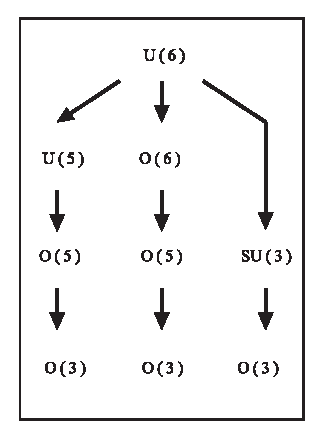
\includegraphics[scale=.65]{figure}
%
% If not, use
%\picplace{5cm}{2cm} % Give the correct figure height and width in cm
%
\caption{Please write your figure caption here}
\label{fig:A1}       % Give a unique label
\end{figure}

% For tables use
%
\begin{table}
\caption{Please write your table caption here}
\label{tab:A1}       % Give a unique label
%
% For LaTeX tables use
%
\begin{tabular}{p{2cm}p{2.4cm}p{2cm}p{4.9cm}}
\hline\noalign{\smallskip}
Classes & Subclass & Length & Action Mechanism  \\
\noalign{\smallskip}\hline\noalign{\smallskip}
Translation & mRNA$^a$  & 22 (19--25) & Translation repression, mRNA cleavage\\
Translation & mRNA cleavage & 21 & mRNA cleavage\\
Translation & mRNA  & 21--22 & mRNA cleavage\\
Translation & mRNA  & 24--26 & Histone and DNA Modification\\
\noalign{\smallskip}\hline\noalign{\smallskip}
\end{tabular}
$^a$ Table foot note (with superscript)
\end{table}
%


\backmatter%%%%%%%%%%%%%%%%%%%%%%%%%%%%%%%%%%%%%%%%%%%%%%%%%%%%%%%

% \Extrachap{Solutions}

\section*{Problems of Chapter~\ref{intro}}

\begin{sol}{prob1}
The solution\index{problems}\index{solutions} is revealed here.
\end{sol}


\begin{sol}{prob2}
\textbf{Problem Heading}\\
(a) The solution of first part is revealed here.\\
(b) The solution of second part is revealed here.
\end{sol}


% \printindex

%%%%%%%%%%%%%%%%%%%%%%%%%%%%%%%%%%%%%%%%%%%%%%%%%%%%%%%%%%%%%%%%%%%%%%

\end{document}





